\documentclass{beamer}
<<<<<<< HEAD

=======
<<<<<<< HEAD:Presentation/projet.tex

=======
>>>>>>> d7b023f (Modification Slides):Presentation/Pres_Slid.tex
>>>>>>> b34d639 (Modification Slides)

\usepackage[utf8]{inputenc} % Required for inputting international characters
\usepackage{bookmark} % Add the bookmark package to handle changed files
\usepackage{booktabs}
\usetheme{CambridgeUS}
\usefonttheme{serif}
\usepackage{opensans}
\usepackage{amsmath}
%----------------------------------------------------------------------------------------
%   PRESENTATION INFORMATION
%----------------------------------------------------------------------------------------
\title{The Discovery of an  Algebraic structure}
\subtitle{CSMI 2024}
\author[ASSIGBE Komi . RAHOUTI Chahid .]{ASSIGBE Komi \and  RAHOUTI Chahid}
\institute[]{University of Strasbourg \\ \smallskip} % Your institution, the optional parameter can be used for the institution shorthand and will appear on the bottom of every slide after author names, while the required parameter is used on the title slide and can include your email address or additional information on separate lines
\date[\today]{Mathematics and applications \\ \today} % Presentation date or conference/meeting name, the optional parameter can contain a shortened version to appear on the bottom of every slide, while the required parameter value is output to the title slide
%----------------------------------------------------------------------------------------
\begin{document}
%----------------------------------------------------------------------------------------
%   TITLE SLIDE
%----------------------------------------------------------------------------------------
\begin{frame}
    \titlepage % Print the title page as the first slide
    \end{frame}
%----------------------------------------------------------------------------------------
%   TABLE OF CONTENTS SLIDE
%----------------------------------------------------------------------------------------


\begin{frame}
<<<<<<< HEAD
<<<<<<< HEAD:Presentation/Pres_Slid.tex
    \titlepage % Print the title page as the first slide
    \end{frame}
=======
<<<<<<<< HEAD:Presentation/projet.tex
<<<<<<< HEAD
	\titlepage % Output the title slide, automatically created using the text entered in the PRESENTATION INFORMATION block above
\end{frame}
>>>>>>> b34d639 (Modification Slides)

%----------------------------------------------------------------------------------------
%	TABLE OF CONTENTS SLIDE
%----------------------------------------------------------------------------------------
<<<<<<< HEAD
<<<<<<< HEAD:Presentation/Pres_Slid.tex
\begin{frame}{Plan}
\tableofcontents
=======
\begin{frame}
<<<<<<< HEAD:Presentation/Pres_Slid.tex
    \frametitle{Table of contents}
    \tableofcontents
>>>>>>> dc0cea6 (Correction of the slides):Presentation/projet.tex
=======
	\frametitle{Presentation overview } % Slide title, remove this command for no title
    \tableofcontents
>>>>>>> 9916fc7 ("verify"):Presentation/projet.tex
=======
    \frametitle{Table of Contents}
    \tableofcontents
    \end{frame}
>>>>>>> 583b858 (Prise en compte des corrections):Presentation/projet.tex
\end{frame}
%----------------------------------------------------------------------------------------
%   PRESENTATION BODY SLIDES
%----------------------------------------------------------------------------------------
=======
\begin{frame}
<<<<<<< HEAD
    \frametitle{Table of contents}
=======
	\frametitle{Presentation overview } % Slide title, remove this command for no title
>>>>>>> 9916fc7 ("verify")
=======
========
<<<<<<< HEAD:Presentation/projet.tex
>>>>>>>> b34d639 (Modification Slides):Presentation/Pres_Slid.tex
    \frametitle{Table of Contents}
>>>>>>> 583b858 (Prise en compte des corrections)
    \tableofcontents
    \end{frame}
\end{frame}
=======
    \titlepage % Print the title page as the first slide
    \end{frame}

>>>>>>> d7b023f (Modification Slides):Presentation/Pres_Slid.tex
%----------------------------------------------------------------------------------------
%   PRESENTATION BODY SLIDES
%----------------------------------------------------------------------------------------
<<<<<<< HEAD
<<<<<<< HEAD:Presentation/projet.tex
=======
=======
<<<<<<< HEAD:Presentation/Pres_Slid.tex
>>>>>>> 99fd072 (Correction of the slides)
\begin{frame}{Plan}
\tableofcontents
=======
\begin{frame}
<<<<<<< HEAD:Presentation/Pres_Slid.tex
    \frametitle{Table of contents}
    \tableofcontents
>>>>>>> dc0cea6 (Correction of the slides):Presentation/projet.tex
=======
	\frametitle{Presentation overview } % Slide title, remove this command for no title
    \tableofcontents
>>>>>>> 9916fc7 ("verify"):Presentation/projet.tex
\end{frame}

%----------------------------------------------------------------------------------------
%	PRESENTATION BODY SLIDES
%----------------------------------------------------------------------------------------

>>>>>>> d7b023f (Modification Slides):Presentation/Pres_Slid.tex
>>>>>>> b34d639 (Modification Slides)
\section{Introduction}


%------------------------------------------------
\subsection{Definition}
\begin{frame}
    \frametitle{Definition}
    What is an Algebraic structure? An algebraic structure consists of a nonempty set A (called the underlying set, carrier set or domain), a collection of operations on A (typically binary operations such as addition and multiplication), and a finite set of identities, known as axioms, that these operations must satisfy.
    Among the multiples algebraic structures, we can name:
    \begin{itemize}
        \item Group
        \item Ring
        \item Field
        \item Vector space
        \item .....
    \end{itemize}
\end{frame}
%------------------------------------------------
<<<<<<< HEAD
<<<<<<< HEAD:Presentation/Pres_Slid.tex

=======
>>>>>>> 583b858 (Prise en compte des corrections):Presentation/projet.tex
=======
<<<<<<< HEAD:Presentation/projet.tex
=======

>>>>>>> d7b023f (Modification Slides):Presentation/Pres_Slid.tex
>>>>>>> b34d639 (Modification Slides)
%---------------------------------------------------------------------------------
\section{Objectives}
\begin{frame}
    \frametitle{The Main Objective}
    Our Main objective consist,  if we are giving a set of data in V, and those data is defined on a regular surface or variety, and we want to know if it is possible to detect a certain algebraic structure using Neural Networks Learning.
\end{frame}
<<<<<<< HEAD
<<<<<<< HEAD
<<<<<<< HEAD:Presentation/Pres_Slid.tex

<<<<<<< HEAD:Presentation/Pres_Slid.tex
<<<<<<< HEAD:Presentation/Pres_Slid.tex
\subsection{First sub objective} 
=======
\subsection{First sub objective}
>>>>>>> 583b858 (Prise en compte des corrections):Presentation/projet.tex
\begin{frame}
    \frametitle{Implementing a Loss function based on the axioms of a
    algebraic structure}
=======
\section{The Objectives}
\begin{frame}
        \frametitle{The First Objective}
>>>>>>> bb4e784 (modification):Presentation/projet.tex
=======
\subsection{First sub objective} 
\begin{frame}
    \frametitle{Implementing a Loss function based on the axioms of a
    algebraic structure}
>>>>>>> dc0cea6 (Correction of the slides):Presentation/projet.tex
=======
=======
>>>>>>> 3b7ca9d (modification)
<<<<<<< HEAD
\subsection{First sub objective}
=======

<<<<<<< HEAD:Presentation/Pres_Slid.tex
<<<<<<< HEAD:Presentation/Pres_Slid.tex
\subsection{First sub objective} 
>>>>>>> cfc4117 (modification)
\begin{frame}
<<<<<<< HEAD
    \frametitle{Implementing a Loss function based on the axioms of a
    algebraic structure}
<<<<<<< HEAD
>>>>>>> b34d639 (Modification Slides)
=======
=======
\section{The Objectives}
\begin{frame}
        \frametitle{The First Objective}
>>>>>>> bb4e784 (modification):Presentation/projet.tex
<<<<<<< HEAD
>>>>>>> 3b7ca9d (modification)
=======
=======
\subsection{First sub objective} 
\begin{frame}
    \frametitle{Implementing a Loss function based on the axioms of a
    algebraic structure}
>>>>>>> dc0cea6 (Correction of the slides):Presentation/projet.tex
>>>>>>> 4e3efa8 (Correction of the slides)
    Let's take an example of a group structure.
    let consider a surface $M \in \mathbb{R}^{n \times n}$
    Like,
    M =
<<<<<<< HEAD
=======
=======
        \frametitle{The First Approch}
=======

\subsection{First sub objective} 
\begin{frame}
<<<<<<< HEAD:Presentation/projet.tex
        \frametitle{The First Objective}
>>>>>>> fec1400 (modification)
=======
    \frametitle{Implementing a Loss function based on the axioms of a
    algebraic structure}
>>>>>>> d7b023f (Modification Slides):Presentation/Pres_Slid.tex
    Let's take an example of a group structure.
    let consider a surface $M \in \mathbb{R}^{n \times n}$
    Like, 
    M = 
>>>>>>> 711340b (mine)
>>>>>>> b34d639 (Modification Slides)
    $\begin{bmatrix}
        \vdots & \vdots & \vdots &\vdots \\
        x_{1} & x_{2} & \cdots & x_{n} \\
        \vdots & \vdots & \vdots &\vdots \\
<<<<<<< HEAD
<<<<<<< HEAD:Presentation/Pres_Slid.tex
    \end{bmatrix}
    $
    with $ x_{i} \in \mathbb{R}^{d}$
=======
    \end{bmatrix}$
    with $ x_{i} \in \mathbb{R}^{d}$
    The question is if we consider M as a group structure, it is possible to find a binary operation ($\circ$) on M such that M is a group.
>>>>>>> 583b858 (Prise en compte des corrections):Presentation/projet.tex
=======
<<<<<<< HEAD:Presentation/projet.tex
    \end{bmatrix}$
<<<<<<< HEAD
    with $ x_{i} \in \mathbb{R}^{d}$
    The question is if we consider M as a group structure, it is possible to find a binary operation ($\circ$) on M such that M is a group.
>>>>>>> b34d639 (Modification Slides)
    \begin{enumerate}
        $\exists e \in M, \forall x \in M, e \circ x = x \circ e = x$
        $\forall x,y \in M, x \circ y = y \circ x$
        $\forall x,y,z \in M, (x \circ y) \circ z = x \circ (y \circ z)$
        $\forall x \in M, \exists -x \in M, x \circ (-x) = (-x) \circ x=e$
<<<<<<< HEAD
=======
=======
    with x_{i} $\in \mathbb{R}^{d}$
    The question is if we consider M as a group structure, it is possible to find a binary operation ($\circ$) on M such that M is a group.
=======
    \end{bmatrix}
    $
    with $ x_{i} \in \mathbb{R}^{d}$
>>>>>>> d7b023f (Modification Slides):Presentation/Pres_Slid.tex
    \begin{enumerate}
        \item $\exists e \in M, \forall x \in M, e \circ x = x \circ e = x$
        \item $\forall x,y \in M, x \circ y = y \circ x$
        \item $\forall x,y,z \in M, (x \circ y) \circ z = x \circ (y \circ z)$
<<<<<<< HEAD:Presentation/projet.tex
        \item $\forall x \in M, \exists -x \in M, x \circ -x = -x \circ x = e$
>>>>>>> 711340b (mine)
=======
        \item $\forall x \in M, \exists -x \in M, x \circ (-x) = (-x) \circ x=e$
>>>>>>> d7b023f (Modification Slides):Presentation/Pres_Slid.tex
>>>>>>> b34d639 (Modification Slides)
    \end{enumerate}

    
\end{frame}
<<<<<<< HEAD
%---------------------------------------------------------------------------------
\subsection{Second sub objective}
\begin{frame}
<<<<<<< HEAD:Presentation/Pres_Slid.tex
<<<<<<< HEAD:Presentation/Pres_Slid.tex
    \frametitle{Find a binary operation on V and a function f }
<<<<<<< HEAD:Presentation/Pres_Slid.tex
=======
    \frametitle{Second Objective}
>>>>>>> bb4e784 (modification):Presentation/projet.tex
=======
    \frametitle{Find a binary operation on V and a function f }
>>>>>>> dc0cea6 (Correction of the slides):Presentation/projet.tex
	Let's take an example of a group structure.
	let consider a set of points  $ V $ and let  $ f: R \rightarrow V $ a one-to-one
	function from $R$ into a codomain $V$. We define the vector addition by
	
<<<<<<< HEAD:Presentation/Pres_Slid.tex
<<<<<<< HEAD:Presentation/Pres_Slid.tex
    $$ x \oplus y = f(f^{-1}(x) + f^{-1}(y)) $$
    $$ \alpha \odot x = f(f^{-1}(x) * \alpha) $$
=======
     $$ x \oplus y = f(f^{-1}(x) + f^{-1}(y)) $$
     $$ \alpha \odot x = f(f^{-1}(x) * \alpha) $$
		
>>>>>>> bb4e784 (modification):Presentation/projet.tex
=======
    $$ x \oplus y = f(f^{-1}(x) + f^{-1}(y)) $$
    $$ \alpha \odot x = f(f^{-1}(x) * \alpha) $$
>>>>>>> dc0cea6 (Correction of the slides):Presentation/projet.tex

	The question is if we consider $V$ as a Vector Space, it is possible to find a binary operation ($\oplus$) and ($\odot$) on $V$ such that $V$ is a Vector Space.
	
=======
=======
<<<<<<< HEAD:Presentation/projet.tex
%---------------------------------------------------------------------------------
\subsection{Second sub objective}
\begin{frame}
<<<<<<< HEAD
    \frametitle{Find a binary operation on V and a function f }
>>>>>>> b34d639 (Modification Slides)
    Let's take an example of a group structure.
    let consider a set of points  $ V $ and let  $ f: R \rightarrow V $ a one-to-one
    function from $R$ into a codomain $V$. We define the vector addition by
    $$ x \oplus y = f(f^{-1}(x) + f^{-1}(y)) $$
    $$ \alpha \odot x = f(f^{-1}(x) * \alpha) $$
    The question is if we consider $V$ as a Vector Space, it is possible to find a binary operation ($\oplus$) and ($\odot$) on $V$ such that $V$ is a Vector Space.
<<<<<<< HEAD
>>>>>>> 583b858 (Prise en compte des corrections):Presentation/projet.tex
\end{frame}
%---------------------------------------------------------------------------------
=======
=======
    \frametitle{Second Objective}
=======


%----------------------------------------------------------------------------------------
%	TITLE SLIDE
%----------------------------------------------------------------------------------------

%---------------------------------------------------------------------------------
\subsection{Second sub objective}
\begin{frame}
<<<<<<< HEAD:Presentation/Pres_Slid.tex
<<<<<<< HEAD:Presentation/Pres_Slid.tex
    \frametitle{Find a binary operation on V and a function f }
<<<<<<< HEAD
>>>>>>> d7b023f (Modification Slides):Presentation/Pres_Slid.tex
=======
=======
    \frametitle{Second Objective}
>>>>>>> bb4e784 (modification):Presentation/projet.tex
<<<<<<< HEAD
>>>>>>> cfc4117 (modification)
=======
=======
    \frametitle{Find a binary operation on V and a function f }
>>>>>>> dc0cea6 (Correction of the slides):Presentation/projet.tex
>>>>>>> 99fd072 (Correction of the slides)
	Let's take an example of a group structure.
	let consider a set of points  $ V $ and let  $ f: R \rightarrow V $ a one-to-one
	function from $R$ into a codomain $V$. We define the vector addition by
	
<<<<<<< HEAD:Presentation/Pres_Slid.tex
<<<<<<< HEAD:Presentation/Pres_Slid.tex
    $$ x \oplus y = f(f^{-1}(x) + f^{-1}(y)) $$
    $$ \alpha \odot x = f(f^{-1}(x) * \alpha) $$
=======
     $$ x \oplus y = f(f^{-1}(x) + f^{-1}(y)) $$
     $$ \alpha \odot x = f(f^{-1}(x) * \alpha) $$
		
>>>>>>> bb4e784 (modification):Presentation/projet.tex
=======
    $$ x \oplus y = f(f^{-1}(x) + f^{-1}(y)) $$
    $$ \alpha \odot x = f(f^{-1}(x) * \alpha) $$
>>>>>>> dc0cea6 (Correction of the slides):Presentation/projet.tex

	The question is if we consider $V$ as a Vector Space, it is possible to find a binary operation ($\oplus$) and ($\odot$) on $V$ such that $V$ is a Vector Space.
	
>>>>>>> fec1400 (modification)
\end{frame}
%---------------------------------------------------------------------------------
<<<<<<< HEAD
=======

%-----------------------------------------------------------------------------------
>>>>>>> fec1400 (modification)
>>>>>>> b34d639 (Modification Slides)
\section{Examples}
\begin{frame}
    \frametitle{Examples}
    \begin{itemize}
        \item Let f be a function from $R$ to $Vect{e_1}$ such that $f(x) = x.e_1$.
        we have $f^{-1}(x) = \lambda$.
            we take x and y in $vect{e_1}$, we have \\
            $x\oplus y = f(f^{-1}(x) + f^{-1}(y)) = x + y$ \\
            $\alpha \odot x = f(f^{-1}(x) * \alpha) = \alpha x$
            \item Let $\beta$ be any positive real number and let $f: \mathbb{R} \rightarrow \mathbb{R}^{+}$be defined by $f(x)=(1 / \beta) e^x$. Then $f$ is a one-to-one function from $\mathbb{R}$ onto the set of positive real numbers, and $f^{-1}(x)=\ln (\beta x)$ for $x>0$. we would define vector addition and scalar multiplication by
            $$
            x \oplus y=\frac{1}{\beta} e^{\ln (\beta x)+\ln (\beta y)}=\beta x y
<<<<<<< HEAD
=======
<<<<<<< HEAD
>>>>>>> b34d639 (Modification Slides)
            $$
            $$
            \alpha \odot x=\frac{1}{\beta} e^{\alpha \ln (\beta x)}=\beta^{\alpha-1} x^\alpha.
            $$
        \end{itemize}
    \end{frame}
<<<<<<< HEAD
<<<<<<< HEAD:Presentation/Pres_Slid.tex
<<<<<<< HEAD:Presentation/Pres_Slid.tex

=======
>>>>>>> 583b858 (Prise en compte des corrections):Presentation/projet.tex
=======
>>>>>>> b34d639 (Modification Slides)
    %-----------------------------------------------------------------------------------
    \section{Tools}
    \begin{frame}{Tools}
        For the implementation of this project, we are going to use :
        \begin{itemize}
            \item Python
            \item Pytorch
            \item Using Neural Networks learning by transforming the axioms of
            an Algebraic structure into a loss to minimize.
            \item using slack to communicate and share Idea
            \item Using Git to share code and work togeether
        \end{itemize}
    \end{frame}
<<<<<<< HEAD
<<<<<<< HEAD:Presentation/Pres_Slid.tex
    \section{Roadmap}
    \begin{frame}{Roadmap}
        \begin{figure}
            \begin{center}
            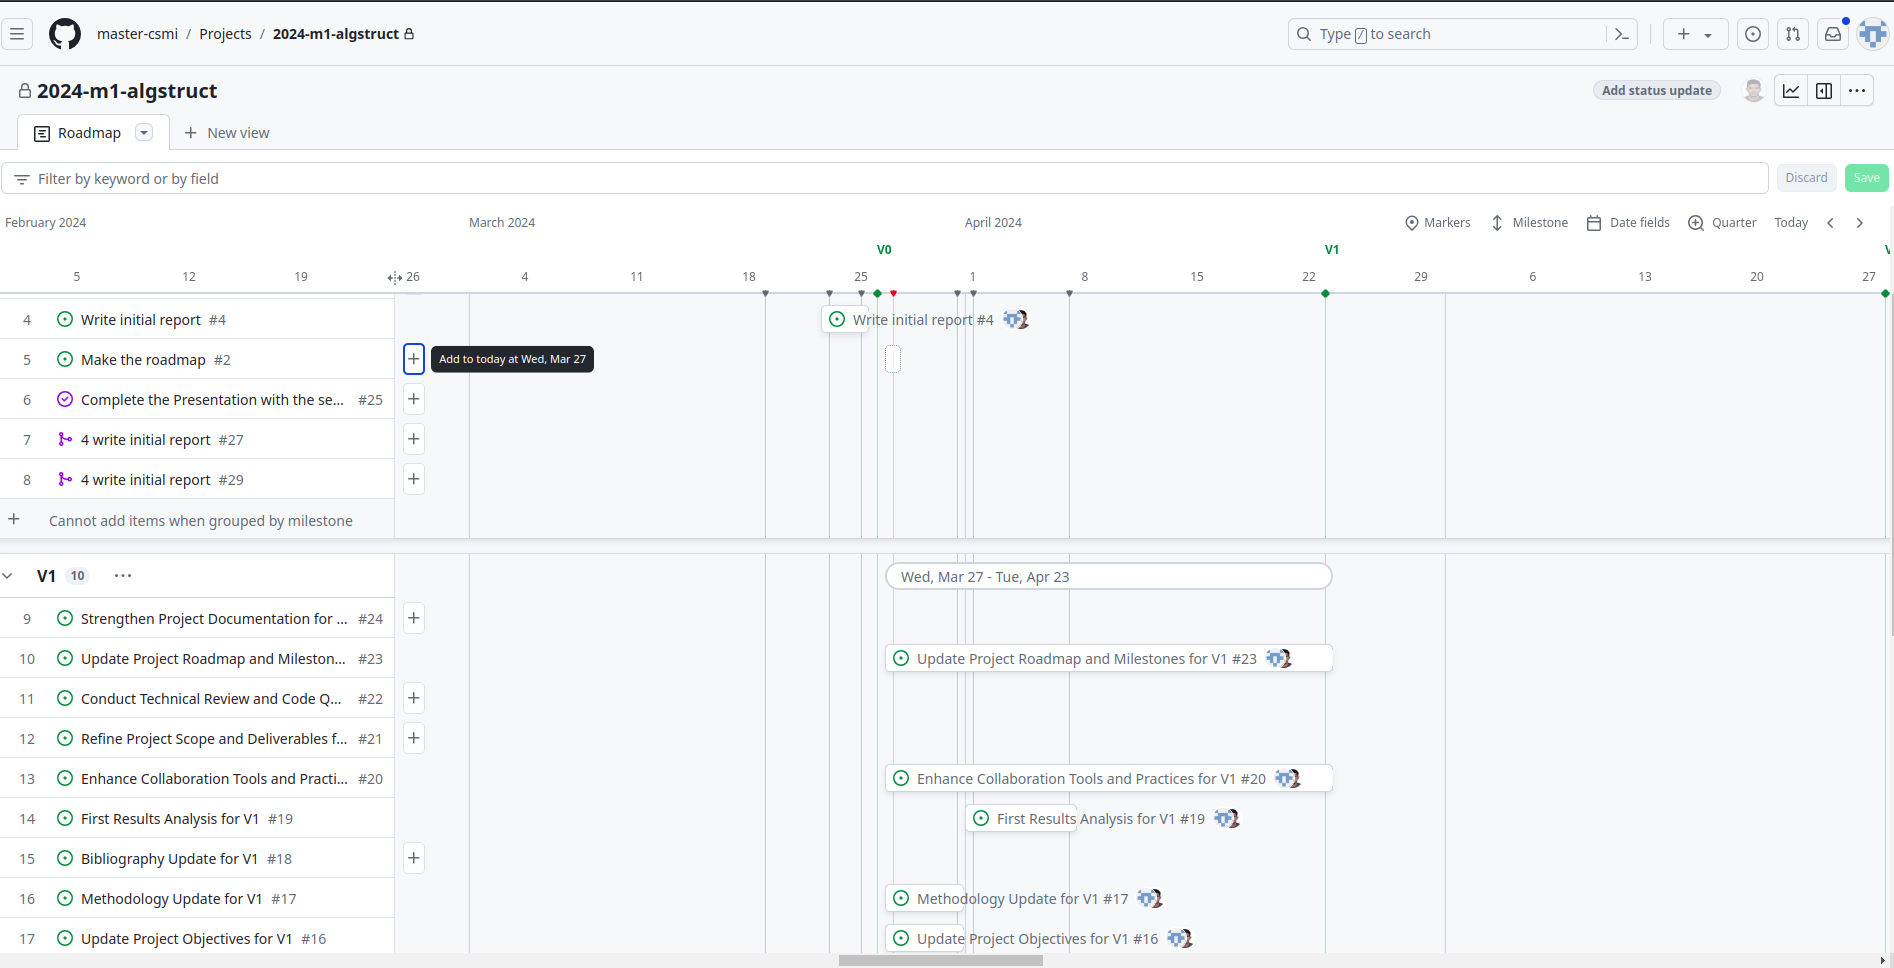
\includegraphics[width=9cm, height=6cm]{roadmap.png}
            %\caption{Roadmap}
            \end{center}
            \end{figure}
        \end{frame}
        
=======
>>>>>>> bb4e784 (modification):Presentation/projet.tex

    %-----------------------------------------------------------------------------------
<<<<<<< HEAD:Presentation/Pres_Slid.tex

<<<<<<< HEAD:Presentation/Pres_Slid.tex
%---------------------------------------------------------------------------------
\end{document}
=======
    
    \section{Application}
    \begin{frame}
        \frametitle{Application}
        Many differential equations encountered 
        in solving have parametric solutions.
         Thus, to find the solution for each 
         parameter, this often requires 
         numerous calculations. To optimize 
         computation and storage times, we 
         define an algebraic structure 
         whereby, if we compute the solution 
         for parameters $\lambda_1$ and $ \lambda_2 $,
         we can deduce $\lambda_3$ ...
         
        \end{frame}
    
    
    
    
    \end{document} 
>>>>>>> bb4e784 (modification):Presentation/projet.tex
=======
=======
\end{document}
=======
            $$ 
            
            $$
            \alpha \odot x=\frac{1}{\beta} e^{\alpha \ln (\beta x)}=\beta^{\alpha-1} x^\alpha.
            $$ 
        \end{itemize}
    \end{frame}
<<<<<<< HEAD:Presentation/Pres_Slid.tex

    %-----------------------------------------------------------------------------------
>>>>>>> b34d639 (Modification Slides)
    \section{Tools}
    \begin{frame}{Tools}
        For the implementation of this project, we are going to use :
        \begin{itemize}
            \item Python
            \item Pytorch
            \item Using Neural Networks learning by transforming the axioms of 
            an Algebraic structure into a loss to minimize.
            \item using slack to communicate and share Idea 
            \item Using Git to share code and work togeether 
        \end{itemize}
    \end{frame}
<<<<<<< HEAD
\end{document} 
>>>>>>> dc0cea6 (Correction of the slides):Presentation/projet.tex
=======
\end{document}
>>>>>>> 583b858 (Prise en compte des corrections):Presentation/projet.tex
=======
    \section{Roadmap}
    \begin{frame}{Roadmap}
        \begin{figure}
            \begin{center}
            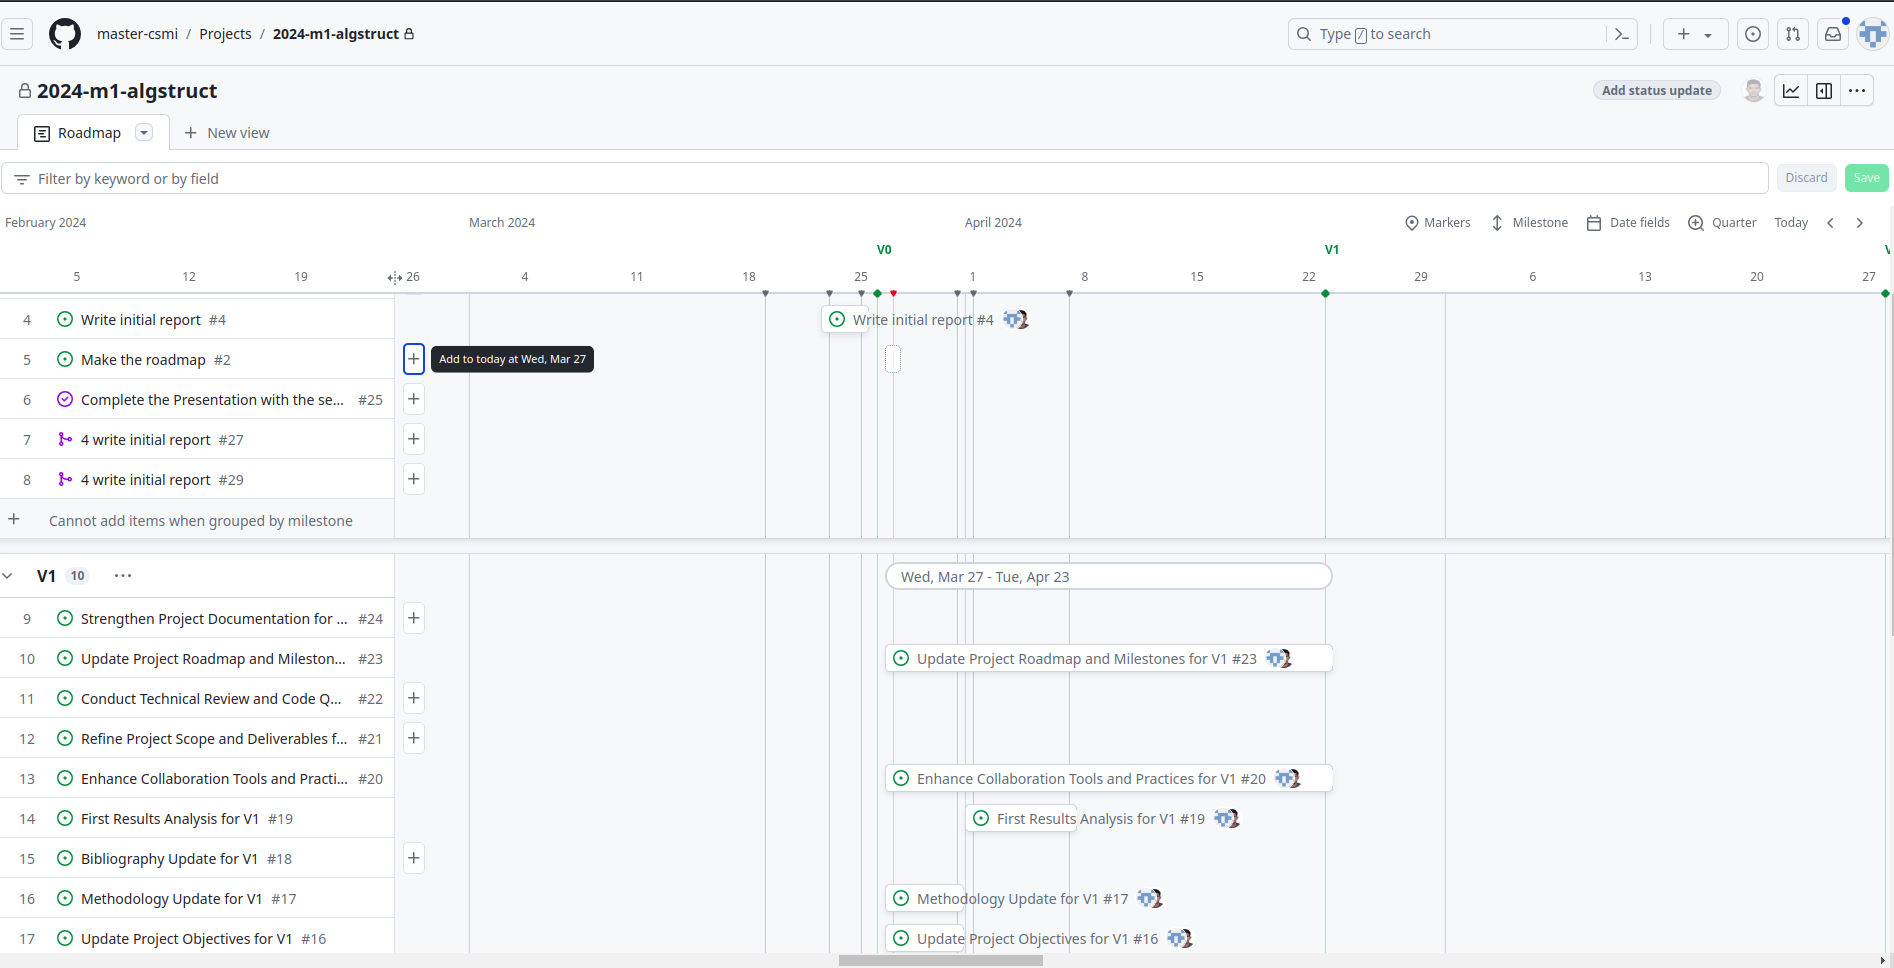
\includegraphics[width=9cm, height=6cm]{roadmap.png}
            %\caption{Roadmap}
            \end{center}
            \end{figure}
        \end{frame}
<<<<<<< HEAD:Presentation/projet.tex
    
    
    
    
    \end{document} 
>>>>>>> fec1400 (modification)
=======
        
=======
>>>>>>> bb4e784 (modification):Presentation/projet.tex

    %-----------------------------------------------------------------------------------
<<<<<<< HEAD:Presentation/Pres_Slid.tex

<<<<<<< HEAD:Presentation/Pres_Slid.tex
%---------------------------------------------------------------------------------
\end{document}
<<<<<<< HEAD
>>>>>>> d7b023f (Modification Slides):Presentation/Pres_Slid.tex
<<<<<<< HEAD
>>>>>>> b34d639 (Modification Slides)
=======
=======
=======
    
    \section{Application}
    \begin{frame}
        \frametitle{Application}
        Many differential equations encountered 
        in solving have parametric solutions.
         Thus, to find the solution for each 
         parameter, this often requires 
         numerous calculations. To optimize 
         computation and storage times, we 
         define an algebraic structure 
         whereby, if we compute the solution 
         for parameters $\lambda_1$ and $ \lambda_2 $,
         we can deduce $\lambda_3$ ...
         
        \end{frame}
    
    
    
    
    \end{document} 
>>>>>>> bb4e784 (modification):Presentation/projet.tex
<<<<<<< HEAD
>>>>>>> cfc4117 (modification)
<<<<<<< HEAD
>>>>>>> 3b7ca9d (modification)
=======
=======
=======
    \section{Tools}
    \begin{frame}{Tools}
        For the implementation of this project, we are going to use :
        \begin{itemize}
            \item Python
            \item Pytorch
            \item Using Neural Networks learning by transforming the axioms of 
            an Algebraic structure into a loss to minimize.
            \item using slack to communicate and share Idea 
            \item Using Git to share code and work togeether 
        \end{itemize}
    \end{frame}
\end{document} 
>>>>>>> dc0cea6 (Correction of the slides):Presentation/projet.tex
>>>>>>> 99fd072 (Correction of the slides)
>>>>>>> 4e3efa8 (Correction of the slides)
